\section{Introduction}
Dealer inventories connect customer order imbalances to risk limits and balance-sheet capacity. Inventory affects optimal dealer pricing and observed position adjustment \citep{ho1981,lyons1995}; dealer capacity also matters for Treasury intermediation \citep{duffie2023}. A position can become large during a holding interval and then return toward its starting value. Monitoring its largest recorded magnitude therefore asks a different question from predicting the endpoint.

We ask when conditional quantile methods forecast a sampled absolute position peak better than simple historical rules. The data comprise an hourly FX market-maker record and weekly Treasury-bill positions. An upper quantile of the peak supplies a monitoring report for future recorded positions. Across these records, historical rules are hard to beat.

Historical headroom and translated-path rules compete with ridge quantile regression and nearest-neighbour quantiles. Matched comparisons use the same completed responses and update schedules. The two pre-specified comparisons pair FX regression with short-history rolling headroom and Treasury regression with long-history frozen headroom.

The paper makes three empirical points. First, the historical benchmark matters for FX forecasts. Regression lowers matched loss by \FXMatchedGain{}\% in the original period and \RWritingMatchedGain{}\% in the earlier 2015 period. It beats the short-history rolling rule only in the original period (Tables~\ref{tab:fx} and~\ref{tab:r6-primary}).

Second, weekly regression struggles against historical headroom. The Treasury-bill main comparison loses \TreasuryOriginalExcess{}\%. Across \PanelSeriesCount{} further weekly series, expanded-menu regression still loses in \PanelExpandedLosses{} of \PanelCellCount{} cells (Figure~\ref{fig:panel}). Conservative one-standard-error selection also leaves large weekly losses (Section~7).

Third, lower pinball loss need not mean fewer breaches. The main FX gain accompanies \FXPrimaryBreaches{} breaches against \FXReferenceBreaches{} for its rolling reference. Neither main comparison dominates across consistent quantile scores (Table~\ref{tab:uv}; Appendix~\ref{app:murphy}). All methods are standard; the contribution is this evidence for the sampled peak, extending the endpoint question studied by \citet{wisniewski2020}.

The paper develops the target and methods before comparing forecast performance. It then examines regularization, error amounts and breaches. Mathematical arguments and implementation details follow in the appendices.

\section{Related literature}
Inventory research provides the economic motivation for position monitoring. \citet{ho1981} model dealer quotes under inventory uncertainty, and \citet{lyons1995} studies inventory and information in FX trading. \citet{duffie2023} connects Treasury-market functioning to dealer capacity.

Financial path extrema and liquidity buffers provide the closest target precedents. MaxVaR measures the worst intermediate portfolio-value loss \citep{boudoukh2004}. \citet{petrunia2019} studies the maximum end-of-day net debit across payment-system participants, and \citet{hoogen2017} models a one-sided maximum cumulative payment deficit. \citet{arjani2020} forecasts a payment-demand/resource ratio. Table~\ref{tab:literature} distinguishes these targets from the absolute peak of a single recorded position series.

Conditional quantile forecasting combines regression with consistent scoring rules. Regression quantiles minimize asymmetric absolute loss \citep{koenker1978}; CAViaR models time-varying conditional quantiles \citep{engle2004}. Volatility-updated historical simulation is an established alternative for financial scenario construction \citep{hull1998,barone1999}. \citet{wisniewski2020} already applies conditional methods and lag/calendar predictors to endpoint intervals in the FX source family. \citet{gneiting2011} formalizes consistent quantile scores, and \citet{ehm2016} represents their comparison through elementary scores. These methods give a common basis for forecasting and scoring the peak response.

\begin{table}[!htbp]
\centering\footnotesize
\caption{Related studies: targets, data, methods and evaluation evidence.}\label{tab:literature}
\begin{tabular}{>{\raggedright\arraybackslash}p{.14\linewidth}>{\raggedright\arraybackslash}p{.20\linewidth}>{\raggedright\arraybackslash}p{.14\linewidth}>{\raggedright\arraybackslash}p{.20\linewidth}>{\raggedright\arraybackslash}p{.20\linewidth}}
\toprule
Study & Target & Data & Method & Evaluation \\
\midrule
Boudoukh et al. (2004) & Worst intermediate portfolio-value loss & Modeled portfolio paths & First-passage formula; discrete simulation & Model-implied MaxVaR/VaR ratios; discrete-monitoring simulation \\
Petrunia et al. (2019) & Largest daily endpoint debit across ACSS participants & ACSS settlement balances & GEV blocks; GPD exceedances & Fitted-versus-empirical quantiles; monthly-updated collateral shortfalls \\
van den Hoogen (2017) & Maximum cumulative negative payment balance & Two ABN AMRO transaction accounts & ACD/UHF-GARCH; Monte Carlo paths & Coverage and independence tests; application details confidential \\
Wisniewski et al. (2020) & Next-hour signed-position interval & One market maker's hourly FX net positions & Quantile/conformal intervals; KNN and other regressions & Two endpoint pinball scores; interval and coverage diagnostics \\
This paper & Two-sided absolute sampled peak quantile & Hourly FX; weekly dealer-position series & Historical rules; QR/KNN on matched histories and updates & Pinball; paired DM; U/V, breaches and elementary scores \\
\bottomrule
\end{tabular}
\par\smallskip\begin{minipage}{\linewidth}\footnotesize Van den Hoogen (2017) specifies coverage and independence tests in Section 5.4; detailed application results in Section 5.5 are confidential, while Chapter 7 provides public out-of-sample summaries.\end{minipage}
\end{table}


The comparison adds three empirical findings for a common sampled position peak. Matched regression gains persist in FX but change sign in Treasury (Tables~\ref{tab:fx}--\ref{tab:treasury}). The earlier FX gain persists against matched history, while the gain over rolling history disappears (Table~\ref{tab:r6-primary}). Wider penalties reduce the weekly panel's median excess loss from \PanelOriginalMedian{}\% to \PanelExpandedMedian{}\%, yet conservative selection still leaves large losses (Figure~\ref{fig:panel}; Section~7). Finally, the main FX score gain accompanies more breaches, and both main Murphy curves cross (Table~\ref{tab:uv}; Appendix~\ref{app:murphy}). These results connect the peak target to benchmark choice, regularization and risk monitoring.

\section{Data and target}
The FX record contains hourly client-flow net positions for one market maker across five liquid currency pairs, as described by \citet{wisniewski2020}. We use the hourly member of the Net Position Time Series Dataset, version two \citep{dataset}. It contains \FXObservationCount{} observations. Adjacent observations are usually an hour apart, with weekend-sized gaps retained in their recorded order. The signed scalar is denominated in source-reported USD. The record belongs to the source family of \citet{wisniewski2020}.

The Treasury input is New York Fed Primary Dealer Statistics series PDPOSGS-B, the aggregate Treasury-bill long position less the short position \citep{nyfeddata}. The weekly Wednesday-close series contains \TreasuryObservationCount{} observations, denominated in USD millions. FR~2004A instructions describe market/fair-value positions on a trade-date basis, including eligible forward and when-issued outright positions, with specified settlement-date treatment for buybacks \citep{fr2004}. Table~\ref{tab:data} gives the chronological splits in calendar dates.

\begin{table}[!htbp]
\centering\footnotesize
\caption{Source-specific chronological budgets. Dates are issue dates; all horizons share the same evaluation issues.}\label{tab:data}
\begin{tabular}{l>{\raggedright\arraybackslash}p{.20\linewidth}>{\raggedright\arraybackslash}p{.20\linewidth}>{\raggedright\arraybackslash}p{.20\linewidth}>{\raggedright\arraybackslash}p{.17\linewidth}}
\toprule
Source & Full record & Validation & Evaluation & $W$ / $d$ \\
\midrule
FX & 2014-02-05 to 2017-01-24 & 2015-10-08 to 2015-12-30 & 2016-01-01 to 2017-01-23 & 720 or 2880 / 24 \\
Treasury & 2013-04-03 to 2026-10-07 & 2019-07-24 to 2020-07-15 & 2021-01-06 to 2026-04-22 & 52 or 260 / 13 \\
\bottomrule
\end{tabular}
\par\smallskip\begin{minipage}{\linewidth}\footnotesize FX has 1,440 validation and 6,625 evaluation issues; Treasury has 52 and 277. The longest validation response completes before evaluation starts. $H$ counts records, preserving recorded FX gaps.\end{minipage}
\end{table}


The target is the largest absolute position over the sampled holding interval. It includes the position known at issue. Let $N_t$ be the signed recorded position and $H$ count subsequent records, with
\begin{equation}\label{eq:target}
B_t=|N_t|,\qquad P_{t,H}=\max_{0\le h\le H}|N_{t+h}|,\qquad G_{t,H}=P_{t,H}-B_t\ge0.
\end{equation}

Endpoint marginals permit different peak distributions. For example, two future magnitudes can each take values zero or one with equal probability. Perfect positive dependence gives maximum one with probability one half; perfect negative dependence gives maximum one with probability one. Figure~\ref{fig:path} illustrates the distinction between an interim peak and the endpoint.

\begin{figure}[htbp]
\centering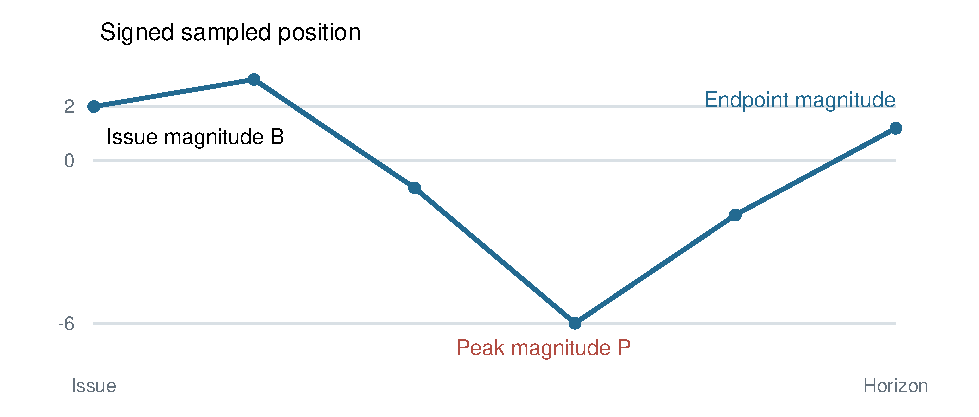
\includegraphics[width=.9\linewidth]{figures/path-target.pdf}
\caption{A sampled path separates the issue magnitude, holding-interval peak and endpoint magnitude. The path is artificial.}\label{fig:path}
\end{figure}

The information set enforces label completion before fitting. Write $\kappa(t)$ for the latest scheduled refit and $W$ for the number of completed training origins. At segment start $t_0$ and refit interval $d$,
\begin{equation}\label{eq:maturity}
\kappa(t)=t_0+d\left\lfloor\frac{t-t_0}{d}\right\rfloor,
\qquad \T_{\kappa,H,W}=\{\kappa-H-W+1,\ldots,\kappa-H\}.
\end{equation}
Every training response ends by $\kappa(t)$. Fitted transforms and coefficients stay fixed between refits, while current query predictors and $B_t$ update at issue. Earlier evaluation outcomes enter training only after completion. Validation and evaluation restart their schedules at their respective segment starts.



\section{Forecasting methods}
\subsection{Historical reports and matched controls}
The historical rules differ in how they anchor completed episodes to the current issue. For each episode $i$, let $\ell_i=\min_h(N_{i+h}-N_i)$ and $u_i=\max_h(N_{i+h}-N_i)$, including $h=0$. At query $x=N_t$, its raw translated peak is $T_i(x)=\max\{x+u_i,-x-\ell_i\}$. For a selected set $A$ of size $m$, $\Q$ denotes its duplicate-preserving order statistic at $j=\lceil(m+1)\tau\rceil$, with $\tau=.95$. Here $F$ denotes historical headroom, $S$ translated paths and $K$ native peaks. The three reports are
\begin{align}\label{eq:historical}
C_t^F&=B_t+\Q\{G_{i,H}:i\in A\},\nonumber\\
C_t^S&=B_t+\Q\{T_i(N_t)-B_t:i\in A\},\\
C_t^K&=\max\{B_t,\Q\{P_{i,H}:i\in A\}\}.\nonumber
\end{align}

Rolling controls use the most recent completed episodes at every issue. Frozen controls use $A=\T_{\kappa,H,W}$, matching the conditional fitting pool and update schedule. The query anchor still updates in a frozen control. Appendix~\ref{app:proofs} gives the finite-array relationships among these constructions.

\subsection{Predictors and training transforms}
The original specification contains 33 predictors. They comprise current and lagged signed levels, current magnitude, two past increment root mean square (RMS) measures, calendar sine/cosine pairs and a gap indicator. The level sequence spans lags zero through 24. RMS uses short and long past-only spans, defined by
\begin{equation}
v_L(i)=\left\{L^{-1}\sum_{q=i-L+1}^{i}(N_q-N_{q-1})^2\right\}^{1/2}.
\end{equation}
The spans are daily and weekly record counts in FX, and six and 26 records in Treasury. All transforms use completed training rows. With training mean $\mu_{\kappa j}$ and population standard deviation $\sigma_{\kappa j}$,
\begin{equation}
z_{i,\kappa j}=\frac{x_{ij}-\mu_{\kappa j}}{\sigma_{\kappa j}},\qquad
s_\kappa=\max\left\{W^{-1}\sum_{i\in\T}G_{i,H},\;10^{-6}W^{-1}\sum_{i\in\T}|N_i|,\;10^{-12}\right\}.
\end{equation}
An exactly constant predictor is centered at its repeated value and assigned scale one. Treasury's calendar and gap coordinates are constant under its weekly sampling. Predictor lookbacks use past observations and can extend beyond the completed-label history. The longer FX RMS reaches before the oldest training origin.

The four-predictor specification uses current signed position, current magnitude and the two past RMS measures. The full specification uses all predictors above. Both select penalties with the same validation rule.

\subsection{Quantile regression and nearest neighbours}
Ridge quantile regression (QR) fits normalized headroom with an unpenalized intercept. For $\rho_\tau(e)=\tau(e)_++(1-\tau)(-e)_+$, it solves
\begin{equation}\label{eq:qr}
\min_{\beta_0,\beta}\frac1W\sum_{i\in\T}\rho_\tau\!\left(\frac{G_{i,H}}{s_\kappa}-\beta_0-z_{i,\kappa}^{\mathsf T}\beta\right)+\frac\lambda2\|\beta\|_2^2,
\end{equation}
and issues $C_t^{QR}=B_t+\max\{0,s_\kappa(\widehat\beta_0+z_{t,\kappa}^{\mathsf T}\widehat\beta)\}$. The original penalty menu is $\{.001,.01,.1\}$. Expanded-menu regression adds the stronger penalties $1$ and $10$. Projection acts on issued reports; the training objective uses the affine headroom prediction. Appendix~\ref{app:ridge} derives the equivalent peak parameterization and its shifted penalty.

As $\lambda\to\infty$, penalized slopes vanish and the unpenalized intercept approaches the set of empirical headroom-quantile minimizers. Write $I_t=B_t+G_{(\lceil W\tau\rceil)}$ for its lower-endpoint reference on the frozen pool. If $W\tau$ is integral, the entire interval between the adjacent order statistics minimizes the intercept-only objective. Thus $I$ is the unique empirical quantile at the shorter Treasury history, while the longer Treasury and both FX histories admit an interval with endpoints $I$ and corrected-rank $F$ (possibly coincident). The different rank conventions can produce different reports.

Nearest-neighbour quantiles (KNN) select standardized predictor rows by a group-balanced Euclidean distance and resolve equal distances by recency. Before computing distance, each lagged-level coordinate is divided by five. Each RMS, hour and weekday coordinate is divided by $\sqrt{2}$. Magnitude and gap retain their standardized scales.

Plain KNN applies the corrected order statistic to selected headrooms. Scaled KNN first divides each selected headroom by a short-run RMS scale and multiplies the resulting quantile by the current scale. The RMS floor is $10^{-6}s_\kappa$. At $k=W$, plain KNN equals frozen $F$ because membership is the full pool.

Standard validation selects the lowest native-unit mean pinball loss. Exact parameter ties favour the larger candidate. Every declared candidate must complete for the cell to be eligible.

\subsection{Residual replay}
Residual replay adds a fitted conditional mean to historical path construction. At each original refit, ordinary least squares estimates an intercept and slope on unique transitions from the union of completed training windows. Ordered residual blocks are replayed from the current position; Appendix~\ref{app:replay} gives the path identity.

\section{Evaluation design}
The two pre-specified comparisons use six-record horizons. The FX comparison pairs long-history regression with the short-history rolling headroom rule. The Treasury comparison pairs regression with its long-history frozen headroom rule. We call these the main comparisons below. The original FX evaluation period was inspected before the conditional methods were specified.

Mean pinball loss measures forecast accuracy, while breach frequency records limit exceedances. For report $C_t$, define the mean underprediction amount $U$ and overprediction amount $V$ by
\begin{equation}\label{eq:score}
U=\frac1M\sum_t(P_{t,H}-C_t)_+,\quad V=\frac1M\sum_t(C_t-P_{t,H})_+,\quad \overline L=.95U+.05V.
\end{equation}
A strict breach occurs when $P_{t,H}>C_t$; equality counts as a nonbreach. Both amounts average over all issues, and headroom is $C_t-B_t$. Scores retain the source units, and percentage changes use the stated reference mean.

Paired loss differences compare unconditional predictive accuracy. For $d_t=L_t^A-L_t^B$, the test statistic is $\bar d/\sqrt{\widehat\Omega/M}$. We estimate $\widehat\Omega$ with Bartlett Newey--West HAC and bandwidth $L=\max\{H,\lfloor4(M/100)^{2/9}\rfloor\}$ \citep{diebold1995,newey1987}. The original short-horizon FX comparisons use ten lags; the other original cells use the horizon. Twice-bandwidth checks and the Harvey--Leybourne--Newbold correction accompany the original comparisons \citep{harvey1997}. The fixed-window interpretation follows \citet{giacomini2006}.

Apart from the two pre-specified comparisons, all p-values are exploratory and unadjusted unless stated. The main comparisons have unadjusted HAC p-values and a two-comparison Bonferroni sensitivity. Table notes identify the remaining Holm-adjusted comparisons \citep{holm1979}.

Coverage diagnostics use the fixed grid $t_0+j(H+1)$, starting at evaluation onset. Its target windows share no recorded observations. The Kupiec test uses every retained hit \citep{kupiec1995}. Christoffersen independence and conditional-coverage likelihood ratios condition on the first hit and use the subsequent transitions \citep{christoffersen1998}. Table~\ref{tab:coverage} reports the resulting tests.

\section{Results}
\subsection{FX: gains depend on history and reference}
Long-history regression beats both six-step FX headroom references. Loss falls by \FXPrimaryGain{}\% against rolling headroom and \FXMatchedGain{}\% against matched frozen headroom. Table~\ref{tab:fx} places this gain beside the short-history forecasts and other conditional methods.

\begin{table}[!htbp]
\centering\small
\caption{FX forecasts matched by horizon and history, with mean pinball losses in source-reported USD millions.}\label{tab:fx}
\begin{tabular}{rrlrrrr}
\toprule
$H$ & $W$ & Report & Mean loss & $\Delta_F$ (\%) & Breach (\%) & $p$ \\
\midrule
6 & 720 & $F$ & 0.443 & +0.000 & 5.011 & -- \\
6 & 720 & $S$ & 0.451 & +1.843 & 3.849 & -- \\
6 & 720 & $K$ & 0.932 & +110.664 & 7.758 & -- \\
6 & 720 & QR & 0.433 & -2.117 & 8.015 & 1.000 \\
6 & 720 & KNN & 0.436 & -1.394 & 4.815 & 1.000 \\
6 & 720 & Scaled KNN & 0.466 & +5.349 & 4.060 & 1.000 \\
6 & 2880 & $F$ & 0.453 & +0.000 & 5.434 & -- \\
6 & 2880 & $S$ & 0.451 & -0.418 & 4.045 & -- \\
6 & 2880 & $K$ & 0.972 & +114.751 & 8.091 & -- \\
6 & 2880 & QR & 0.386 & -14.767 & 5.675 & $<0.001$ \\
6 & 2880 & KNN & 0.411 & -9.302 & 4.815 & 0.016 \\
6 & 2880 & Scaled KNN & 0.426 & -5.795 & 4.121 & 1.000 \\
24 & 720 & $F$ & 0.787 & +0.000 & 6.445 & -- \\
24 & 720 & $S$ & 0.755 & -4.078 & 4.362 & -- \\
24 & 720 & $K$ & 1.206 & +53.135 & 11.049 & -- \\
24 & 720 & QR & 1.035 & +31.504 & 13.947 & 0.066 \\
24 & 720 & KNN & 0.836 & +6.197 & 7.592 & 1.000 \\
24 & 720 & Scaled KNN & 0.897 & +13.886 & 6.642 & 1.000 \\
24 & 2880 & $F$ & 0.763 & +0.000 & 5.389 & -- \\
24 & 2880 & $S$ & 0.759 & -0.525 & 4.408 & -- \\
24 & 2880 & $K$ & 1.240 & +62.440 & 8.936 & -- \\
24 & 2880 & QR & 0.735 & -3.758 & 8.015 & 1.000 \\
24 & 2880 & KNN & 0.770 & +0.837 & 6.883 & 1.000 \\
24 & 2880 & Scaled KNN & 0.848 & +11.085 & 5.962 & 1.000 \\
\bottomrule
\end{tabular}
\par\smallskip\begin{minipage}{\linewidth}\footnotesize Relative changes use each report's frozen $F$; conditional p-values use Holm over the remaining 71 matched conditional-versus-$F/S/K$ contrasts. Dashes mark historical contrasts, self-comparisons or exact full-pool KNN identities; identical losses enter the adjustment with p-value one.\end{minipage}
\end{table}


Short-history regression offers little six-step improvement. Its matched gain is \FXShortGain{}\%, with $p=\FXShortP{}$. Table~\ref{tab:fx} contrasts this weak result with the long-history gain.

The short-history 24-step regression loses, even under the expanded penalty menu. Its loss rises by \FXShortLongExcess{}\%, and both menus select $\lambda=\FXShortLongPenalty{}$. The identical selected reports show that menu expansion leaves this failure intact.

The 24-step FX comparison gives a small, imprecise gain. Regression lowers loss by \FXLegacyGain{}\% against rolling translated paths, with $p=\FXLegacyP{}$. This gain is concentrated in the partial \FXTailYear{} tail, while the six-step main gain has the same direction in each issue year.

\FloatBarrier
\subsection{Treasury: original regression loses to historical headroom}
Original Treasury regression loses to matched historical headroom. The main comparison raises loss by \TreasuryOriginalExcess{}\%, with $p=\TreasuryPrimaryP{}$. All original regression and scaled-neighbour cells lose to their own frozen headroom references (Table~\ref{tab:treasury}).

The Treasury loss increase accompanies more breaches. Their count rises from \TreasuryReferenceBreaches{} to \TreasuryOriginalBreaches{} in the main comparison. Table~\ref{tab:treasury} shows that the adverse score result extends across both histories and horizons.

\begin{table}[!htbp]
\centering\small
\caption{Treasury original reports, matched by horizon and history. Loss is in source-reported USD millions.}\label{tab:treasury}
\begin{tabular}{rrlrrrr}
\toprule
$H$ & $W$ & Report & Mean loss & $\Delta_F$ (\%) & Breach (\%) & $p_{\rm Holm}$ \\
\midrule
6 & 52 & $F$ & 2779.054 & +0.000 & 3.971 & -- \\
6 & 52 & $S$ & 2786.620 & +0.272 & 3.971 & -- \\
6 & 52 & $K$ & 2574.098 & -7.375 & 10.108 & -- \\
6 & 52 & QR & 5095.519 & +83.354 & 30.325 & 0.114 \\
6 & 52 & KNN & 2779.054 & +0.000 & 3.971 & -- \\
6 & 52 & Scaled KNN & 4208.293 & +51.429 & 3.249 & 0.013 \\
6 & 260 & $F$ & 2758.665 & +0.000 & 10.108 & -- \\
6 & 260 & $S$ & 2707.244 & -1.864 & 10.108 & -- \\
6 & 260 & $K$ & 2287.758 & -17.070 & 10.469 & -- \\
6 & 260 & QR & 4159.673 & +50.786 & 19.495 & 0.320 \\
6 & 260 & KNN & 2663.561 & -3.447 & 10.108 & 1.000 \\
6 & 260 & Scaled KNN & 3127.173 & +13.358 & 8.303 & 1.000 \\
24 & 52 & $F$ & 3715.693 & +0.000 & 11.913 & -- \\
24 & 52 & $S$ & 3652.379 & -1.704 & 11.913 & -- \\
24 & 52 & $K$ & 5017.741 & +35.042 & 25.271 & -- \\
24 & 52 & QR & 12165.574 & +227.411 & 47.653 & 0.983 \\
24 & 52 & KNN & 3715.693 & +0.000 & 11.913 & -- \\
24 & 52 & Scaled KNN & 5625.667 & +51.403 & 11.552 & 0.231 \\
24 & 260 & $F$ & 2480.306 & +0.000 & 4.332 & -- \\
24 & 260 & $S$ & 2478.871 & -0.058 & 4.332 & -- \\
24 & 260 & $K$ & 2301.476 & -7.210 & 24.188 & -- \\
24 & 260 & QR & 5204.760 & +109.843 & 30.325 & 1.000 \\
24 & 260 & KNN & 2257.963 & -8.964 & 4.693 & 1.000 \\
24 & 260 & Scaled KNN & 4137.264 & +66.805 & 2.888 & $<0.001$ \\
\bottomrule
\end{tabular}
\par\smallskip\begin{minipage}{\linewidth}\footnotesize Every relative change uses its own frozen $F$. Holm adjustment covers the original 72 matched conditional-versus-$F/S/K$ contrasts. Dashes mark self-references, historical contrasts outside that family, or the exact full-pool KNN identity. Identical-loss cells receive input one solely for conservative family bookkeeping. Percentages and loss are computed before display rounding.\end{minipage}
\end{table}


The plain nearest-neighbour forecast reproduces historical headroom at the short Treasury history. Validation selects the full eligible pool at both horizons. At the longer history and horizon, its full-sample gain reverses on the twelve-point nonoverlap grid. Both reports have two breaches on that grid.

Coverage diagnostics reinforce Treasury regression's adverse breach record. The two Treasury grids contain \TreasuryShortGridCount{} and \TreasuryLongGridCount{} observations. Table~\ref{tab:coverage} puts the regression tests beside historical headroom and the FX comparison.

\begin{table}[!htbp]
\centering\small
\caption{Six-step coverage diagnostics on the fixed nonoverlap grid.}\label{tab:coverage}
\begin{tabular}{lrrrrrr}
\toprule
Report & $n$ & Breaches & Rate (\%) & $p_{\rm POF}$ & $p_{\rm IND}$ & $p_{\rm CC}$ \\
\midrule
FX QR & 947 & 50 & 5.280 & 0.695 & 0.388 & 0.636 \\
Treasury QR & 40 & 7 & 17.500 & 0.004 & 0.775 & 0.014 \\
Treasury $F$ & 40 & 4 & 10.000 & 0.199 & 0.338 & 0.262 \\
\bottomrule
\end{tabular}
\par\smallskip\begin{minipage}{\linewidth}\footnotesize POF uses every retained hit. IND and CC condition on the first hit; their likelihoods therefore use the subsequent transitions consistently. Values are asymptotic reference p-values for equality/independence nulls. Complete grids and the preserved earlier initialization convention are in the inference supplement.\end{minipage}
\end{table}


\FloatBarrier
\subsection{What changes when histories, predictors and penalties change?}\label{sec:decomposition}
Penalty expansion accounts for most of the Treasury score improvement in the ordered comparison. The main regression's excess loss falls from \TreasuryOriginalExcess{}\% to \TreasuryExpandedExcessFine{}\%. Table~\ref{tab:e3} holds the original labels and update schedule fixed while expanding the penalty menu.

The two predictor sets give similar Treasury scores under the common menu. Full regression has \TreasuryFeatureChange{}\% higher loss than four-predictor regression, with $p=0.685$. Table~\ref{tab:decomp} separates this predictor-set comparison from the final return to the smaller penalty menu.

The FX gain survives the wider penalty menu. Switching from four predictors to the full set lowers long-history loss by \FXFeaturesGain{}\%, with adjusted $p<.001$. Its selected reports equal those from the original full regression (Table~\ref{tab:e3}).

Stronger Treasury shrinkage leaves the breach count above historical headroom. At the main Treasury setting, expanded-menu regression has 32 breaches against 28 for the historical rule. Table~\ref{tab:e3} also places the ordinary intercept-only quantile beside each regression.

\begin{table}[!htbp]
\centering\footnotesize
\caption{E3: the full predictor set under a shared wider ridge menu. Score changes are relative to frozen $F$ (percent).}\label{tab:e3}
\begin{tabular}{lrrrrrrr}
\toprule
Source & $H$ & $W$ & $\lambda_{33+}$ & Original 33 & Four+ & 33+ & $p_{4+\to33+}$ \\
\midrule
FX & 6 & 720 & 0.01 & -2.117 & +1.476 & -2.117 & 0.193 \\
FX & 6 & 2880 & 0.01 & -14.767 & -4.289 & -14.767 & $<.001$ \\
FX & 24 & 720 & 0.01 & +31.504 & +16.513 & +31.504 & 0.023 \\
FX & 24 & 2880 & 0.001 & -3.758 & -2.894 & -3.758 & 0.813 \\
Treasury & 6 & 52 & 10 & +83.354 & -2.589 & -3.244 & 0.142 \\
Treasury & 6 & 260 & 1 & +50.786 & +2.166 & +3.434 & 0.685 \\
Treasury & 24 & 52 & 10 & +227.411 & +5.955 & +4.340 & 0.013 \\
Treasury & 24 & 260 & 10 & +109.843 & +0.110 & -0.193 & 0.857 \\
\bottomrule
\end{tabular}
\par\smallskip\begin{minipage}{\linewidth}\footnotesize Plus denotes the common menu $\{.001,.01,.1,1,10\}$. Original 33 retains its published smaller menu. Each feature set selects its own penalty by the same validation rule; the comparison is between tuning procedures, not a fixed-penalty feature effect. The last column is an unadjusted exploratory HAC p-value. All eight cells and all 40 candidates completed. The separate 28-comparison E3 adjustment, HLN and doubled-bandwidth results are retained in the supplement.\end{minipage}
\end{table}

\begin{table}[!htbp]
\centering\footnotesize
\caption{Ordered six-step loss changes from historical rules to original regression.}\label{tab:decomp}
\begin{tabular}{l>{\raggedright\arraybackslash}p{.43\linewidth}rrrr}
\toprule
Source & Change & Step (\%) & Initial (pp) & $p_{\rm DM}$ & $p_{\rm HLN}$ \\
\midrule
FX & Rolling $F_{720}$$\to$Frozen $F$ & +0.190 & +0.190 & 0.297 & 0.297 \\
FX & Frozen $F_{720}$$\to$Frozen $F_{2880}$ & +2.277 & +2.281 & 0.143 & 0.143 \\
FX & Frozen $F$$\to$four-predictor regression & -4.289 & -4.395 & 0.010 & 0.010 \\
FX & four-predictor regression$\to$expanded-menu regression & -10.947 & -10.736 & $<.001$ & $<.001$ \\
FX & expanded-menu regression$\to$original regression & +0.000 & +0.000 & -- & -- \\
Treasury & Frozen $F$$\to$four-predictor regression & +2.166 & +2.166 & 0.178 & 0.188 \\
Treasury & four-predictor regression$\to$expanded-menu regression & +1.242 & +1.269 & 0.685 & 0.691 \\
Treasury & expanded-menu regression$\to$original regression & +45.779 & +47.352 & 0.006 & 0.007 \\
\bottomrule
\end{tabular}
\par\smallskip\begin{minipage}{\linewidth}\footnotesize Step percentages use each preceding loss and compound; initial percentage points share the chain's starting loss and add. The last Treasury step restores the smaller penalty menu, dashes mark identical losses, and paired tests are unadjusted.\end{minipage}
\end{table}


\begin{figure}[htbp]
\centering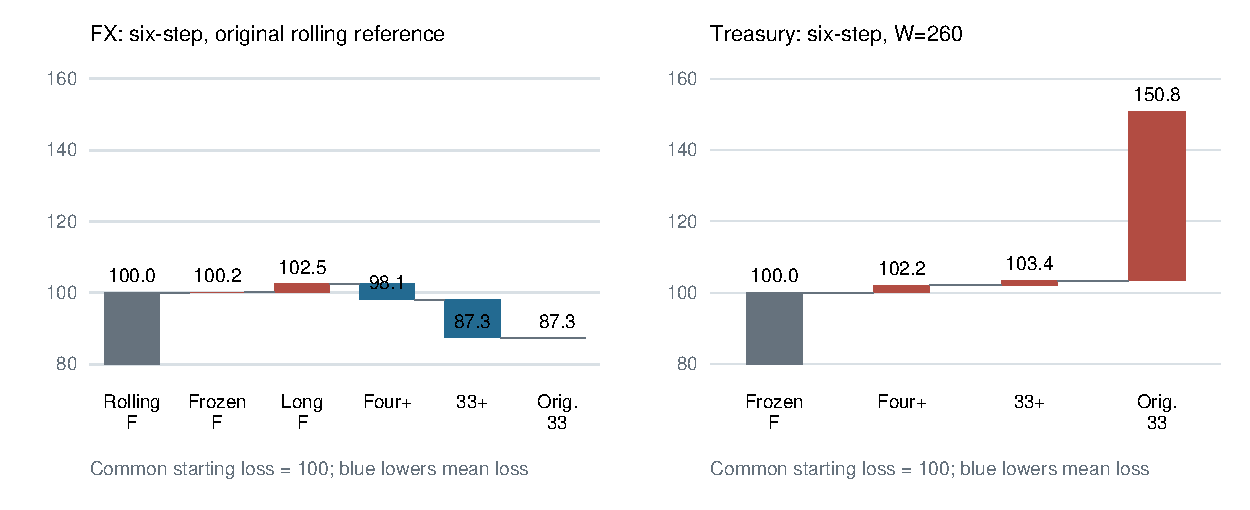
\includegraphics[width=\linewidth]{figures/decomposition.pdf}
\caption{Successive procedure changes in the six-step comparisons. Each increment uses the chain's common starting loss, so the displayed increments sum to the total. Table~\ref{tab:decomp} gives the corresponding paired tests.}\label{fig:waterfall}
\end{figure}

Expanded-menu regression still loses in most additional weekly cells. It loses in \PanelExpandedLosses{} of \PanelCellCount{} cells. Figure~\ref{fig:panel} covers \PanelSeriesCount{} further dealer-position series across the same histories and horizons.

Menu expansion nevertheless reduces the typical weekly deterioration substantially. Median excess loss falls from \PanelOriginalMedian{}\% to \PanelExpandedMedian{}\%. Figure~\ref{fig:panel} shows both versions against historical headroom for every cell.

Two of the three pre-set panel predictions fail. The number of losing cells falls from 45 to 34. Appendix~\ref{app:repro} gives the fixed prediction thresholds and all three outcomes.

\begin{figure}[htbp]
\centering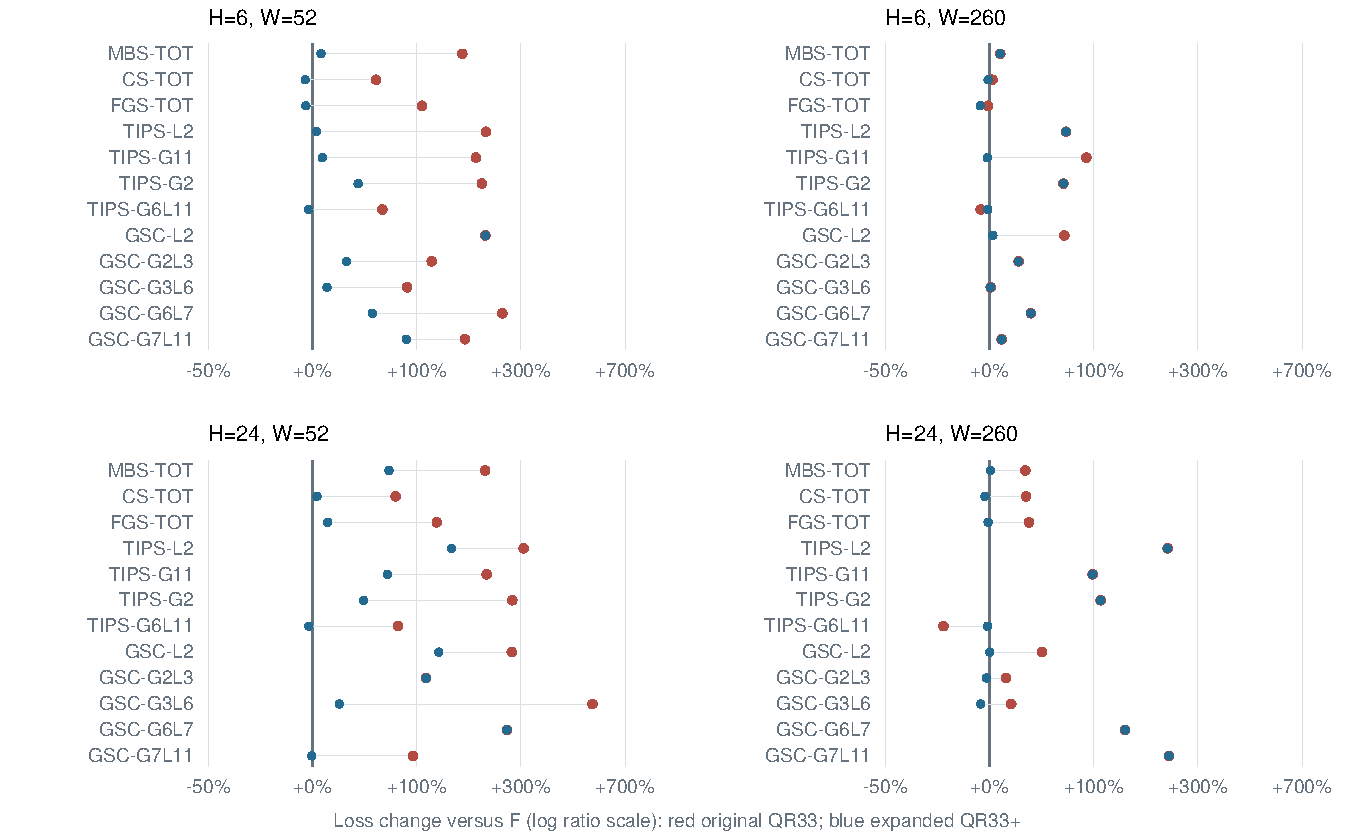
\includegraphics[width=\linewidth]{figures/panel-menu.pdf}
\caption{Original and expanded-menu regression compared with matched historical headroom in every additional weekly panel cell. Relative losses use a logarithmic ratio scale; zero marks the historical reference. Row labels omit the common series prefix.}\label{fig:panel}
\end{figure}

\section{Robustness and score interpretation}
Residual replay improves some scores while increasing breaches. It lowers loss in 5/8 cells against each matched historical reference. Breaches rise against translated paths in every cell and against headroom in 5/8 (Table~\ref{tab:robustness}).

Residual replay improves the main Treasury score against both historical references. Loss falls by 20.4\% against headroom and 18.9\% against translated paths. Its 31 breaches exceed the headroom rule's 28.

Residual replay also beats most Treasury regression reports. It beats expanded-menu regression in 3/4 Treasury cells, including a 23.0\% reduction at the main setting. It beats original regression in every Treasury cell; Appendix~\ref{app:replay} gives the path construction.

The historical quantile rank changes both reports and rankings. Corrected headroom uses $\lceil(m+1)\tau\rceil$, while the ordinary empirical quantile uses $\lceil m\tau\rceil$. The ranks differ in the short Treasury pool, and nearest-neighbour headroom equals frozen headroom when both use the full pool and the same rank.

The main FX gain improves both mean error amounts while increasing breaches. The breach count rises from \FXReferenceBreaches{} to \FXPrimaryBreaches{}. Table~\ref{tab:uv} separates the underprediction and overprediction amounts from their frequency.

The 24-step FX gain trades greater underprediction for less overprediction. Its ranking reverses above an underprediction/overprediction weight ratio of \FXLegacyCrossing{}. For fixed reports, $J_\omega=\omega U+V$ gives this comparison, with the original score corresponding to $\omega=19$.

Both main comparisons change ranking across consistent quantile scores. Each elementary-score curve takes positive and negative values. Appendix~\ref{app:murphy} and Figure~\ref{fig:murphy} show these crossings.

\begin{table}[!htbp]
\centering\small
\caption{Error components and strict breaches for the original comparisons.}\label{tab:uv}
\begin{tabular}{>{\raggedright\arraybackslash}p{.35\linewidth}rrrr}
\toprule
Comparison & $\Delta U$ & $\Delta V$ & Crossing $\omega$ & Breaches A/B \\
\midrule
FX six-step main comparison & -0.010 & -0.921 & -- & 376/332 \\
FX six-step matched & -0.030 & -0.776 & -- & 376/360 \\
FX 24-step comparison & +0.168 & -3.463 & 20.631 & 531/287 \\
Treasury main comparison & +1736.223 & -4968.078 & 2.861 & 54/28 \\
\bottomrule
\end{tabular}
\par\smallskip\begin{minipage}{\linewidth}\footnotesize A denotes regression and B its stated historical reference; amounts are source-reported USD millions, and negative differences favor regression. A missing crossing means both components share a sign; $\omega$ represents fixed-report preferences.\end{minipage}
\end{table}


\begin{figure}[htbp]
\centering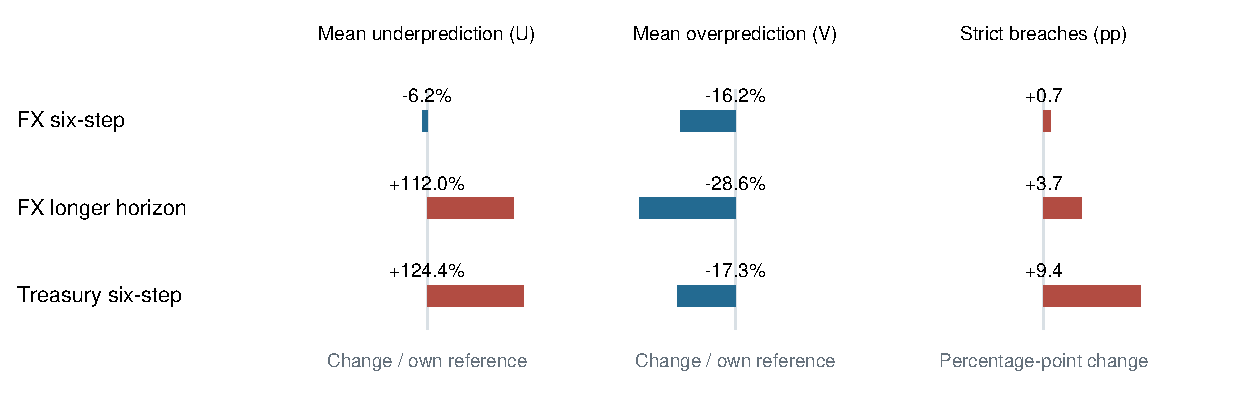
\includegraphics[width=\linewidth]{figures/error-components.pdf}
\caption{Changes in underprediction amounts, overprediction amounts and strict breaches for the original comparisons. Each amount panel scales its own reference to 100; breaches use percentage-point changes. The two sources retain their distinct position units.}\label{fig:errors}
\end{figure}

Fitted quantile reports can cross across horizons even though realized peaks increase. Long-history Treasury regression crosses on about \TreasuryHorizonCrossing{}\% of common issues. Raising a longer-horizon report to remove a crossing can worsen its score, as Appendix~\ref{app:replay} illustrates.

\begin{table}[!htbp]
\centering\footnotesize
\caption{Compact robustness summary; the complete original outputs are retained.}\label{tab:robustness}
\begin{tabular}{>{\raggedright\arraybackslash}p{.19\linewidth}>{\raggedright\arraybackslash}p{.47\linewidth}>{\raggedright\arraybackslash}p{.23\linewidth}}
\toprule
Check & Finding & Interpretation \\
\midrule
AR residual replay & Lower loss than $F$ in 5/8 and $S$ in 5/8; more breaches than $S$ in 8/8 & Lower loss than QR33+ in 3/4 Treasury cells \\
Rank convention & Ordinary versus corrected rank changes some finite reports; full-pool identities persist & Report construction matters \\
Fixed linear weights & FX short-horizon components both fall; longer-horizon crossing near the original weight & Mean score and breach count differ \\
Horizon order & Targets are ordered; fitted reports can cross & Separate fits need an explicit reconciliation criterion \\
\bottomrule
\end{tabular}
\end{table}


The earlier-period exercise keeps the forecast target and uses shorter weekly histories. Each weekly cell has \RWritingWeeklyN{} evaluation points, and the FX comparison has \RWritingFXN{} origins. The FX span is about \RWritingFXWeeks{} calendar weeks; the weekly set includes Treasury bills and the additional panel. The earlier origins were first evaluated here, although the rules were designed after seeing the original results.

The conservative one-standard-error rule favours stronger shrinkage when validation losses are close. It selects the most shrunk candidate within one paired-loss HAC standard error of the best, including the intercept-only option. The rule adapts \citet{hastie2009} to paired forecast losses.

All three pre-set success criteria fail for this conservative rule. Weekly excess loss has median \RWeeklyTwoMedian{}\% and worst \RWeeklyTwoWorst{}\%. The worst cell is Treasury bills at the 24-record horizon.

Both the protection and median-improvement requirements fail. The fixed protection limits are \RProtectionWorstLimit{}\% for the worst cell and \RProtectionMedianLimit{}\% for the median. Standard validation has a lower median excess loss of \RWeeklyZeroMedian{}\%, and \RWeeklyTwoLargeLosses{} conservative-rule cells exceed the worst-cell limit.

Frequent selection of the intercept-only option coexists with large weekly losses. The conservative rule chooses it in \RWritingISelected{} of \RWritingWeeklyCells{} cells. The ordinary empirical quantile and corrected-rank headroom use different order statistics, as Section~4 explains.

The conservative rule also gives up more than half the eligible FX gain. Long-history loss changes by \RFXLongTwoChange{}\%, against \RFXLongZeroChange{}\% under standard validation. This misses the pre-set gain-retention criterion.

Rolling cross-validation produces two failed FX cells. A required validation candidate fails to complete in those cells. Both failures occur at the short history, one at each horizon.

The earlier FX period repeats the matched gain but reverses the rolling-reference comparison. The loss changes are $-\RWritingMatchedGain{}\%$ and $+\RWritingOriginalExcess{}\%$, respectively. Table~\ref{tab:r6-primary} pairs the same regression reports with the two historical references.

The earlier rolling-reference difference is statistically imprecise. The matched and rolling comparisons have $p=\RWritingMatchedP{}$ and $p=\RWritingOriginalP{}$, respectively. Table~\ref{tab:r6-primary} identifies each reference and its inference settings.

The earlier Treasury comparison retains the adverse regression direction. The short-window version raises loss by \RWritingTreasuryExcess{}\% at $W=52$. Table~\ref{tab:r6-primary} uses the same weekly evaluation issues for both reports.

\begin{table}[htbp]
\centering\small
\begin{tabular}{p{.31\linewidth}p{.29\linewidth}rr}
\toprule
Retrospective structure & Historical reference & Selected $\lambda$ & $\Delta$ (\%) \\
\midrule
Treasury bill QR, $W=52$ analogue & Frozen $F$, $W=52$, $d=13$ & 0.1 & +144.3 \\
FX QR, $W=2880$ & Rolling $F$, $W=720$, $d=1$ & 0.01 & +3.2 \\
\bottomrule
\end{tabular}
\caption{Original comparison structures on the R6 retrospective six-step origins, with the original three-penalty menu retuned on the earlier validation segment. $\Delta$ is QR mean pinball relative to the stated reference; positive is worse. The Treasury row is a short-window structural analogue, not an exact replication of the original $W=260$ primary. Original primaries remain unchanged.}\label{tab:r6-primary}
\end{table}


\section{Implications for position monitoring}\label{sec:implications}
\textbf{Benchmark against historical headroom.} Compare conditional reports with historical headroom on the same completed labels and update schedule. Original regression loses all Treasury-bill comparisons and most additional weekly panel cells.

\textbf{Default to corrected-rank headroom in short weekly samples.} Use the corrected-rank historical rule as the starting point for these short samples. Wider penalties and conservative one-standard-error selection leave large losses, while the ordinary empirical quantile's excess loss reaches \RWeeklyIWorst{}\%.

\textbf{Report breaches with the score.} Show underprediction amounts, overprediction amounts and breach counts alongside pinball loss. The main FX gain accompanies more breaches, so a lower score alone misses part of the monitoring outcome.

\section{Discussion and limitations}\label{sec:limits}
The two data sources describe different dealer-position records. The FX client-flow series samples part of one dealer's activity, while Treasury aggregates positions across reporting dealers. Both omit movements between recorded observations. Treasury observations use a downloaded vintage indexed by economic date, and aggregation can hide offsetting positions and valuation effects.

The comparisons describe forecasting performance within these records. The original FX evaluation period was inspected before the conditional methods were specified. The procedure comparisons are not causal and do not identify the effects of individual predictors. Shared reporting and overlapping positions also connect the additional weekly series.

Forecast scores and breach counts answer different monitoring questions. Their interpretation depends on the response, rank convention and chosen score. The study provides no conditional-coverage guarantee and measures no trading, collateral or funding benefit.

\section{Conclusion}
Simple historical rules are hard to beat when forecasting peaks of dealer net positions. In hourly FX, regression improves on matched historical headroom in both evaluation periods (\FXMatchedGain{}\% and \RWritingMatchedGain{}\%). Its gain over the short-history rolling rule appears only in the original period; earlier loss increases \RWritingOriginalExcess{}\%.

On weekly positions, stronger regularization narrows regression's gap, but \PanelExpandedLosses{} of \PanelCellCount{} panel cells still lose. Conservative one-standard-error selection also leaves large weekly losses. Lower pinball loss and fewer breaches diverge in the main FX comparison, and both main Murphy curves cross. Position-limit model selection should therefore compare historical rules and report both error amounts and breaches. These retrospective findings from two sources provide no conditional-coverage guarantee and measure no trading or funding benefit.
